\documentclass[conference,compsoc]{IEEEtran}
\usepackage[pdftex]{graphicx}
\usepackage{pgf}
\usepackage{tikz}
\usetikzlibrary{arrows,automata}
\ifCLASSOPTIONcompsoc
  % IEEE Computer Society needs nocompress option
  % requires cite.sty v4.0 or later (November 2003)
  \usepackage[nocompress]{cite}
\else
  % normal IEEE
  \usepackage{cite}
\fi
\ifCLASSINFOpdf
  % declare the path(s) where your graphic files are
  % \graphicspath{{../pdf/}{../jpeg/}}
  % and their extensions so you won't have to specify these with
  % every instance of \includegraphics
  % \DeclareGraphicsExtensions{.pdf,.jpeg,.png}
\else
  % or other class option (dvipsone, dvipdf, if not using dvips). graphicx
  % will default to the driver specified in the system graphics.cfg if no
  % driver is specified.
  % \usepackage[dvips]{graphicx}
  % declare the path(s) where your graphic files are
  % \graphicspath{{../eps/}}
  % and their extensions so you won't have to specify these with
  % every instance of \includegraphics
  % \DeclareGraphicsExtensions{.eps}
\fi
\hyphenation{op-tical net-works semi-conduc-tor}

\begin{document}
\title{Modern AI for games individual assignment}
\author{\IEEEauthorblockN{Sigurt Bladt Dinesen}
\IEEEauthorblockA{IT University of Copenhagen\\
sidi@itu.dk}
}
\maketitle
\IEEEpeerreviewmaketitle

\section{Introduction}
This report describes the implementation of three Ms. Pac-Man controllers (agents):
\begin{enumerate}
	\item A finite state automata whose transitions are determined by a genetic
		algorithm (section \ref{sec:GA}).
	\item An agent trained with temporal difference learning (section
		\ref{sec:qlearning}).
	\item An agent controlled by monte carlo tree search (section \ref{sec:mcts})
\end{enumerate}


\section{Agent: FSM and Evolutionary Computation}
\label{sec:GA}

The first agent (henceforth GA) was submitted to the first part of the competition, and consists of three parts:

\begin{enumerate}
\item Three pre-implemented strategies for the agent.
\item A state machine that transitions between pre-implemented strategies based
	on game state.
\item A genetic algorithm that determines threshold values for the transitions
	in the state machine.
\end{enumerate}

The GA agent hence has two "phases". First; a learning phase where the genetic
algorithm finds good parameters for the state transitions. This happens before
the game is played, and is not part of the agents actual behaviour.

The second phase is the actual play, where a strategy is determined by the state
machine -- based on the parameters found by the genetic algorithm -- and played out.
\subsection{The pre-implemented strategies}
The three pre-implemented strategies are as follows:

 \texttt{FIND\_PILL} strategy, in which the agent determines the location of the
nearest pill in the maze, and follows the shortest path to it.

A \texttt{FLEE} strategy, in which the shortest-path lengths between the agent
and all potentially threatening ghosts\footnotemark\ are determined.
Potentially threatening ghosts are considered \textit{actual} threats if they
are less than a certain distance from the agent. This distance threshold is
determined by the genetic algorithm. The agent makes a move away from all
threatening ghosts if possible, otherwise the agent makes a random valid move.

A \texttt{HUNT\_GHOST} strategy, in which the agent determines the location of
the closest edible ghost (again, by shortest-path length), and moves towards
that position.

\begin{figure}[hbtp]
	\framebox{
		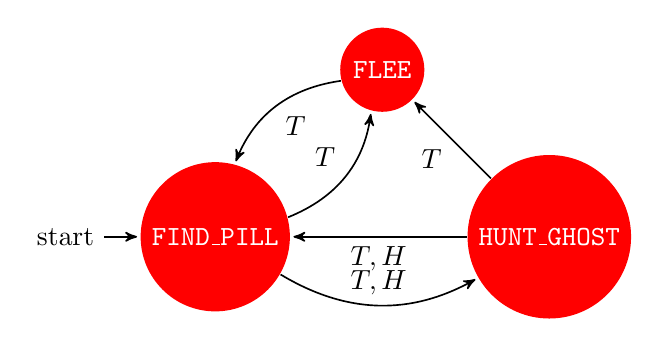
\begin{tikzpicture}[->,>=stealth',shorten >=1pt,auto,node distance=3.0cm,
                    semithick]
  \tikzstyle{every state}=[fill=red,draw=none,text=white]

  \node[initial,state] (fp)                    {\texttt{FIND\_PILL}};
  \node[state]         (f) [above right of=fp] {\texttt{FLEE}};
  \node[state]         (hg) [below right of=f] {\texttt{HUNT\_GHOST}};

  \path (fp) edge [bend right] node {$T$} (f)
             edge [bend right] node {$T,H$} (hg)
        (f) edge [bend right] node {$T$} (fp)
        (hg) edge node {$T$} (f)
        (hg) edge node {$T,H$} (fp);
\end{tikzpicture}

	}
\caption{Diagram of the state machine used by the GA agent}
\end{figure}

\subsection{Genetic Algorithm}
The genetic algorithm simply determines two threshold values: the distance
between the agent and the closest threatening ghost that will cause a transition
to the \texttt{FLEE} strategy ($T$), and the distance to the closest edible
ghost that will cause a transition to the \texttt{HUNT\_GHOST} strategy ($H$).

Note that transitions to and from the \texttt{HUNT\_GHOST} state technically
depend on both parameters, as transitions to \texttt{FLEE} are always considered
first, the $H$ threshold is only considered if the value for $T$ does not cause
a transition.

The scores earned by this agent range between 2000 and 9000 points, usually
lying around 5000 points.

\footnotetext{A ghost is considered a potential threat if it is not
blue, and is not inside the ghost lair.}



\section{Agent: Temporal Difference Learning with Q-Learning}
\label{sec:qlearning}
I tried two approaches for training an agent with temporal difference learning.
First, I simply tried training the agent by letting it play Ms. Pac-Man,
adjusting expectations according to actual game scores. Then I tried training it
by giving it a high reward for actions that the GA agent would have picked in the
same state, and low rewards for different actions. Neither of these approaches
where particularly successful.

The score earned by this agent usually lies around 2000 points.
Interestingly, weather I train the agent on half a million game-runs or 3
million game runs made little to no difference.




\section{Agent: Monte Carlo Tree Search}
\label{sec:mcts}

This agent uses monte carlo tree seach to choose its actions. It uses the
actual \textit{Game} class as state representation, and is hence not as
susceptible to issues arising from an incomplete state definition as the other
agents. However, its foresight is noticeably limited by the search-depth it can
achieve within the allocated timeslot.

The agent receives a complete description of the state, and produces a single
action as output. Although the state description is complete, the search space
is artificially limited, in order to decrease the space size. The agent will
expand nodes in the tree, by adding child-nodes consisting if
\textit{interesting} neighbours. This idea comes from Tom Pepel's
paper\cite{tompepels}. From the agents position, a depth-first-search is
performed through the maze, looking for the first interesting position
encountered on any path. A position in the maze is considered interesting if;
\begin{itemize}
	\item it is a junction (a node with 3 or more neighbours), or
	\item it is a turn (a node that cannot fit on a line with all its neighbours), or
	\item it contains a power pill, or
	\item it contains a ghost
\end{itemize}

Including ghost positions as separate states makes it easier for the agent to
hunt them, as eating a ghost is no longer an incident that occurs when moving
between two positions, but a state in the search space by it self.

This goes for both the tree policy and the default policy, with the only
difference being that the default policy picks child-states at random, where the
tree policy uses the UCT formula.



\section{Implementations}
The implementations are handed in as three different source directories, one for
each agent. This is not particularly clean, as share some code (e.g. the pacman
source code), but it was the easiest, as they share code with modifications.

Each directory contains a \texttt{src} folder, which in turn contains one or
more folders with the prefix "sidi". These package contain the agents.

The agent implementations are all based on the source code provided to us for
the weekly labs, I did not write any of it from scratch, but they contain
extensive modifications.

\begin{thebibliography}{1}
\bibitem{tompepels}
Tom Pepels, \emph{Enhancements for Monte-Carlo Tree Search in Ms Pac-Man} June 19 2012
\end{thebibliography}

\end{document}
